\documentclass[a4paper]{article}

\def\npart {III}
\def\nterm {Lent}
\def\nyear {2018}
\def\nlecturer {J.\ Miller}
\def\ncourse {Schramm--Loewner Evolutions}
\def\nofficial {https://statslab.cam.ac.uk/~jpm205/teaching/lent2018/}

% Imports
\ifx \nextra \undefined
  \usepackage[pdftex,
    hidelinks,
    pdfauthor={Dexter Chua},
    pdfsubject={Cambridge Maths Notes: Part \npart\ - \ncourse},
    pdftitle={Part \npart\ - \ncourse},
  pdfkeywords={Cambridge Mathematics Maths Math \npart\ \nterm\ \nyear\ \ncourse}]{hyperref}
  \title{Part \npart\ - \ncourse}
\else
  \usepackage[pdftex,
    hidelinks,
    pdfauthor={Dexter Chua},
    pdfsubject={Cambridge Maths Notes: Part \npart\ - \ncourse\ (\nextra)},
    pdftitle={Part \npart\ - \ncourse\ (\nextra)},
  pdfkeywords={Cambridge Mathematics Maths Math \npart\ \nterm\ \nyear\ \ncourse\ \nextra}]{hyperref}

  \title{Part \npart\ - \ncourse \\ {\Large \nextra}}
\fi

\author{Lectured by \nlecturer \\\small Notes taken by Dexter Chua}
\date{\nterm\ \nyear}

\usepackage{alltt}
\usepackage{amsfonts}
\usepackage{amsmath}
\usepackage{amssymb}
\usepackage{amsthm}
\usepackage{booktabs}
\usepackage{caption}
\usepackage{enumitem}
\usepackage{fancyhdr}
\usepackage{graphicx}
\usepackage{mathtools}
\usepackage{microtype}
\usepackage{multirow}
\usepackage{pdflscape}
\usepackage{pgfplots}
\usepackage{siunitx}
\usepackage{tabularx}
\usepackage{tikz}
\usepackage{tkz-euclide}
\usepackage[normalem]{ulem}
\usepackage[all]{xy}

\pgfplotsset{compat=1.12}

\pagestyle{fancyplain}
\lhead{\emph{\nouppercase{\leftmark}}}
\ifx \nextra \undefined
  \rhead{
    \ifnum\thepage=1
    \else
      \npart\ \ncourse
    \fi}
\else
  \rhead{
    \ifnum\thepage=1
    \else
      \npart\ \ncourse\ (\nextra)
    \fi}
\fi
\usetikzlibrary{arrows}
\usetikzlibrary{decorations.markings}
\usetikzlibrary{decorations.pathmorphing}
\usetikzlibrary{positioning}
\usetikzlibrary{fadings}
\usetikzlibrary{intersections}
\usetikzlibrary{cd}

\newcommand*{\Cdot}{\raisebox{-0.25ex}{\scalebox{1.5}{$\cdot$}}}
\newcommand {\pd}[2][ ]{
  \ifx #1 { }
    \frac{\partial}{\partial #2}
  \else
    \frac{\partial^{#1}}{\partial #2^{#1}}
  \fi
}

% Theorems
\theoremstyle{definition}
\newtheorem*{aim}{Aim}
\newtheorem*{axiom}{Axiom}
\newtheorem*{claim}{Claim}
\newtheorem*{cor}{Corollary}
\newtheorem*{defi}{Definition}
\newtheorem*{eg}{Example}
\newtheorem*{fact}{Fact}
\newtheorem*{law}{Law}
\newtheorem*{lemma}{Lemma}
\newtheorem*{notation}{Notation}
\newtheorem*{prop}{Proposition}
\newtheorem*{thm}{Theorem}

\renewcommand{\labelitemi}{--}
\renewcommand{\labelitemii}{$\circ$}
\renewcommand{\labelenumi}{(\roman{*})}

\let\stdsection\section
\renewcommand\section{\newpage\stdsection}

% Strike through
\def\st{\bgroup \ULdepth=-.55ex \ULset}

% Maths symbols
\newcommand{\bra}{\langle}
\newcommand{\ket}{\rangle}

\newcommand{\N}{\mathbb{N}}
\newcommand{\Z}{\mathbb{Z}}
\newcommand{\Q}{\mathbb{Q}}
\renewcommand{\H}{\mathbb{H}}
\newcommand{\R}{\mathbb{R}}
\newcommand{\C}{\mathbb{C}}
\newcommand{\Prob}{\mathbb{P}}
\renewcommand{\P}{\mathbb{P}}
\newcommand{\E}{\mathbb{E}}
\newcommand{\F}{\mathbb{F}}
\newcommand{\cU}{\mathcal{U}}
\newcommand{\RP}{\mathbb{RP}}
\newcommand{\CP}{\mathbb{CP}}

\newcommand{\ph}{\,\cdot\,}

\DeclareMathOperator{\sech}{sech}
\DeclareMathOperator{\cosech}{cosech}
\DeclareMathOperator{\cosec}{cosec}

\DeclareMathOperator{\covol}{covol}
\DeclareMathOperator{\vol}{vol}

\let\Im\relax
\let\Re\relax
\DeclareMathOperator{\Im}{Im}
\DeclareMathOperator{\Re}{Re}
\DeclareMathOperator{\im}{im}
\DeclareMathOperator{\image}{image}
\DeclareMathOperator{\Ann}{Ann}

\DeclareMathOperator*{\res}{res}
\DeclareMathOperator{\Res}{Res}
\DeclareMathOperator{\Ind}{Ind}

\DeclareMathOperator{\tr}{tr}
\DeclareMathOperator{\diag}{diag}
\DeclareMathOperator{\rank}{rank}
\DeclareMathOperator{\card}{card}
\DeclareMathOperator{\spn}{span}
\DeclareMathOperator{\adj}{adj}

\DeclareMathOperator{\erf}{erf}
\DeclareMathOperator{\erfc}{erfc}

\DeclareMathOperator{\ord}{ord}
\DeclareMathOperator{\Sym}{Sym}

\DeclareMathOperator{\sgn}{sgn}
\DeclareMathOperator{\orb}{orb}
\DeclareMathOperator{\stab}{stab}
\DeclareMathOperator{\ccl}{ccl}

\DeclareMathOperator{\lcm}{lcm}
\DeclareMathOperator{\hcf}{hcf}

\DeclareMathOperator{\Int}{Int}
\DeclareMathOperator{\id}{id}

\DeclareMathOperator{\betaD}{beta}
\DeclareMathOperator{\gammaD}{gamma}
\DeclareMathOperator{\Poisson}{Poisson}
\DeclareMathOperator{\binomial}{binomial}
\DeclareMathOperator{\multinomial}{multinomial}
\DeclareMathOperator{\Bernoulli}{Bernoulli}
\DeclareMathOperator{\like}{like}

\DeclareMathOperator{\var}{var}
\DeclareMathOperator{\cov}{cov}
\DeclareMathOperator{\bias}{bias}
\DeclareMathOperator{\mse}{mse}
\DeclareMathOperator{\corr}{corr}

\DeclareMathOperator{\otp}{otp}
\DeclareMathOperator{\dom}{dom}

\DeclareMathOperator{\Root}{Root}
\DeclareMathOperator{\supp}{supp}
\DeclareMathOperator{\rel}{rel}
\DeclareMathOperator{\Hom}{Hom}
\DeclareMathOperator{\Aut}{Aut}
\DeclareMathOperator{\Gal}{Gal}
\DeclareMathOperator{\Mat}{Mat}
\DeclareMathOperator{\End}{End}
\DeclareMathOperator{\Char}{char}
\DeclareMathOperator{\ev}{ev}
\DeclareMathOperator{\St}{St}
\DeclareMathOperator{\Lk}{Lk}
\DeclareMathOperator{\disc}{disc}
\DeclareMathOperator{\Isom}{Isom}
\DeclareMathOperator{\length}{length}
\DeclareMathOperator{\energy}{energy}
\DeclareMathOperator{\area}{area}
\DeclareMathOperator{\Syl}{Syl}
\DeclareMathOperator{\cl}{cl}
\DeclareMathOperator{\fix}{fix}

\newcommand{\GL}{\mathrm{GL}}
\newcommand{\SL}{\mathrm{SL}}
\newcommand{\PGL}{\mathrm{PGL}}
\newcommand{\PSL}{\mathrm{PSL}}
\newcommand{\PSU}{\mathrm{PSU}}
\newcommand{\Or}{\mathrm{O}}
\newcommand{\SO}{\mathrm{SO}}
\newcommand{\U}{\mathrm{U}}
\newcommand{\SU}{\mathrm{SU}}

\renewcommand{\d}{\mathrm{d}}
\newcommand{\D}{\mathrm{D}}

\tikzset{->/.style = {decoration={markings,
                                  mark=at position 1 with {\arrow[scale=2]{latex'}}},
                      postaction={decorate}}}
\tikzset{<-/.style = {decoration={markings,
                                  mark=at position 0 with {\arrowreversed[scale=2]{latex'}}},
                      postaction={decorate}}}
\tikzset{<->/.style = {decoration={markings,
                                   mark=at position 0 with {\arrowreversed[scale=2]{latex'}},
                                   mark=at position 1 with {\arrow[scale=2]{latex'}}},
                       postaction={decorate}}}
\tikzset{->-/.style = {decoration={markings,
                                   mark=at position #1 with {\arrow[scale=2]{latex'}}},
                       postaction={decorate}}}
\tikzset{-<-/.style = {decoration={markings,
                                   mark=at position #1 with {\arrowreversed[scale=2]{latex'}}},
                       postaction={decorate}}}

\tikzset{circ/.style = {fill, circle, inner sep = 0, minimum size = 3}}
\tikzset{mstate/.style={circle, draw, blue, text=black, minimum width=0.7cm}}

\definecolor{mblue}{rgb}{0.2, 0.3, 0.8}
\definecolor{morange}{rgb}{1, 0.5, 0}
\definecolor{mgreen}{rgb}{0.1, 0.4, 0.2}
\definecolor{mred}{rgb}{0.5, 0, 0}

\def\drawcirculararc(#1,#2)(#3,#4)(#5,#6){%
    \pgfmathsetmacro\cA{(#1*#1+#2*#2-#3*#3-#4*#4)/2}%
    \pgfmathsetmacro\cB{(#1*#1+#2*#2-#5*#5-#6*#6)/2}%
    \pgfmathsetmacro\cy{(\cB*(#1-#3)-\cA*(#1-#5))/%
                        ((#2-#6)*(#1-#3)-(#2-#4)*(#1-#5))}%
    \pgfmathsetmacro\cx{(\cA-\cy*(#2-#4))/(#1-#3)}%
    \pgfmathsetmacro\cr{sqrt((#1-\cx)*(#1-\cx)+(#2-\cy)*(#2-\cy))}%
    \pgfmathsetmacro\cA{atan2(#2-\cy,#1-\cx)}%
    \pgfmathsetmacro\cB{atan2(#6-\cy,#5-\cx)}%
    \pgfmathparse{\cB<\cA}%
    \ifnum\pgfmathresult=1
        \pgfmathsetmacro\cB{\cB+360}%
    \fi
    \draw (#1,#2) arc (\cA:\cB:\cr);%
}
\newcommand\getCoord[3]{\newdimen{#1}\newdimen{#2}\pgfextractx{#1}{\pgfpointanchor{#3}{center}}\pgfextracty{#2}{\pgfpointanchor{#3}{center}}}

\def\Xint#1{\mathchoice
   {\XXint\displaystyle\textstyle{#1}}%
   {\XXint\textstyle\scriptstyle{#1}}%
   {\XXint\scriptstyle\scriptscriptstyle{#1}}%
   {\XXint\scriptscriptstyle\scriptscriptstyle{#1}}%
   \!\int}
\def\XXint#1#2#3{{\setbox0=\hbox{$#1{#2#3}{\int}$}
     \vcenter{\hbox{$#2#3$}}\kern-.5\wd0}}
\def\ddashint{\Xint=}
\def\dashint{\Xint-}

\renewcommand\D{\mathbb{D}}
\DeclareMathOperator\hcap{hcap}
\newcommand\SLE{\mathrm{SLE}}
\newcommand\rad{\mathrm{Rad}}
\newcommand\dist{\mathrm{dist}}

\usepackage[first=0,last=1, seed=173]{lcg}

\begin{document}
\maketitle
{\small
\setlength{\parindent}{0em}
\setlength{\parskip}{1em}
Schramm--Loewner Evolution (SLE) is a family of random curves in the plane, indexed by a parameter $\kappa \geq 0$. These non-crossing curves are the fundamental tool used to describe the scaling limits of a host of natural probabilistic processes in two dimensions, such as critical percolation interfaces and random spanning trees. Their introduction by Oded Schramm in 1999 was a milestone of modern probability theory.

The course will focus on the definition and basic properties of SLE. The key ideas are conformal invariance and a certain spatial Markov property, which make it possible to use It\^o calculus for the analysis. In particular we will show that, almost surely, for $\kappa \leq 4$ the curves are simple, for $4 \leq \kappa < 8$ they have double points but are non-crossing, and for $\kappa \geq 8$ they are space-filling. We will then explore the properties of the curves for a number of special values of $\kappa$ (locality, restriction properties) which will allow us to relate the curves to other conformally invariant structures.

The fundamentals of conformal mapping will be needed, though most of this will be developed as required. A basic familiarity with Brownian motion and It\^o calculus will be assumed but recalled.
}
\tableofcontents

\section{Introduction}
\section{Conformal transformations}
\subsection{Conformal transformations}
\begin{defi}[Conformal map]\index{conformal map}
  Let $U, V$ be domains in $\C$. We say a map $f: U \to V$ is \emph{conformal} if it is a bijection.
\end{defi}

We will write \term{$\D$} for the open unit disk, and \term{$\H$} for the upper half plane. An important theorem about conformal maps is the following:
\begin{thm}[Riemann mapping theorem]
  Let $U$ be a simply connected domain with $U \not= \C$ and $z \in U$ be any point. Then there exists a unique conformal transformation $f: \D \to U$ such that $f(0) = z$, and $f'(0)$ is real and positive.
\end{thm}
We shall not prove this theorem, as it is a standard result. An immediate corollary is that any two simply connected domains that are distinct from $\C$ are conformally equivalent.

\begin{eg}
  Take $U = \D$. Then for $z \in \D$, the map promised by the Riemann mapping theorem is
  \[
    f(w) = \frac{w + z}{1 + \bar{z} w}.
  \]
  In general, every conformal transformation $f: \D \to \D$ is of the form
  \[
    f(w) = \lambda \frac{w + z}{1 + \bar{z}w}
  \]
  for some $|\lambda| = 1$ and $z \in \D$.
\end{eg}

\begin{eg}
  The map $f: \H \to \D$ given by
  \[
    f(z) = \frac{z - i}{z + i},
  \]
  is a conformal transformation, with inverse
  \[
    g(w) = \frac{i(1 + w)}{1 - w}.
  \]
  In general, the conformal transformations $\H \to \H$ consist of maps of the form
  \[
    f(z) = \frac{az + b}{c z + d}
  \]
  with $a, b, c, d \in \R$ and $ad - bc \not= 0$.
\end{eg}

\begin{eg}
  For $t \geq 0$, we let $H_t = \H \setminus [0, 2\sqrt{t} i]$. The map $H_t \to \H$ given by
  \[
    z \mapsto \sqrt{z^2 + 4t}
  \]
  is a conformal transformation. Observe that this map satisfies
  \[
    |g_t(z) - z| = |\sqrt{z^2 + 4t} - z| \to 0\text{ as } z \to \infty.
  \]
  So $g_t(z) \sim z$ for large $z$.

  Observe also that the family $g_t(z)$ satisfies the ODE
  \[
    \frac{\partial g}{\partial t} = \frac{2}{g_t(z)},\quad g_0(z) = z.
  \]
  We can think of these functions $g_t$ as being generated by the curve $\gamma(t) = 2 \sqrt{t}i$, where for each $t$, the function $g_t$ is the conformal transformation that sends $\H \setminus \gamma([0, t])$ to $\H$ (satisfying $|g_t(z) - z| \to \infty$). Given the set of functions $g_t$, we can recover the curve $\gamma$ as follows --- for each $z \in \H$, we can ask what is the minimum $t$ such that $g_t$ is not defined on $z$. By ODE theorems, there is a solution up till the point when $g_t(z) = 0$, in which case the denominator of the right hand side blows up. Call this time $\tau(z)$. We then see that for each $t$, there is a unique $z$ such that $\tau(z) = t$, and we have $\gamma(t) = z$.

  More generally, suppose $\gamma$ is any simple (i.e.\ non-self-intersecting) curve in $\H$ starting from $0$. Then for each $t$, we can let $g_t$ be the unique conformal transformation that maps $\H \setminus \gamma([0, rt])$ to $\H$ with $|g_t(z) - z| \to \infty$ as above (we will later see such a map exists). Then Loewner's theorem says there is a continuous, real-valued function $W$ such that
  \[
    \frac{\partial g_t}{\partial t} = \frac{2}{g_t(z) - W_t},\quad g_0(z) = z.
  \]
  This is the \term{chordal Loewner equation}. We can turn this around --- given a function $W_t$, what is the corresponding curve $\gamma(t)$? If $W = 0$, then $\gamma(t) = 2\sqrt{t}i$. More excitingly, if we take $W = \sqrt{\kappa} B$, where $B$ is a standard Brownian motion, and then interpret this equation in stochastic calculus, then we obtain $\SLE_\kappa$.
\end{eg}
\subsection{Brownian motion and harmonic functions}
Recall that a function $f = u + iv$ is holomorphic iff it satisfies the \term{Cauchy--Riemann equations}
\[
  \frac{\partial u}{\partial x} = \frac{\partial v}{\partial y},\quad \frac{\partial u}{\partial y} = - \frac{\partial v}{\partial x}.
\]
This in particular implies that both $u$ and $v$ are \term{harmonic}.
\begin{defi}[Harmonic function]\index{harmonic function}
  A function $f: \R^k \to \R$ is \emph{harmonic} if it is $C^2$ and
  \[
    \Delta f = \left(\frac{\partial^2}{\partial x_1^2} + \cdots + \frac{\partial^2}{\partial x_k^2}\right) f = 0.
  \]
\end{defi}
Indeed, we can calculate
\[
  \frac{\partial^2 u}{\partial x^2} + \frac{\partial^2 u}{\partial y^2} = \frac{\partial}{\partial x} \frac{\partial v}{\partial y} + \frac{\partial}{\partial y} \left(- \frac{\partial v}{\partial x}\right) = 0.
\]
In Advanced Probability, we saw that Brownian motion is very closely related to harmonic functions. We say a process $B = B^1 + i B^2$ is a \term{complex Brownian motion} if $(B^1, B^2)$ is a standard Brownian motion in $\R^2$.

Recall some results from Advanced Probability:
\begin{thm}
  Let $u$ be a harmonic function on a bounded domain $D$ which is continuous on $\bar{D}$. For $z \in D$, let $\P_z$ be the law of a complex Brownian motion starting from $z$, and let $\tau$ be the first hitting time of $D$. Then
  \[
    u(z) = \E_z[u(B_\tau)].\fakeqed
  \]
\end{thm}

\begin{cor}[Mean value property]\index{mean value property}
  If $u$ is a harmonic function, then, whenever it makes sense, we have
  \[
    u(z) = \frac{1}{2\pi} \int_0^{2\pi} u(z + re^{i\theta})\;\d \theta.\qedhere
  \]
\end{cor}
\begin{cor}[Maximum principle]\index{maximum principle}
  Let $u$ be harmonic in a domain $D$. If $u$ attains its maximum at an interior point in $D$, then $u$ is constant.
\end{cor}

\begin{cor}[Maximum modulus principle]\index{maximum modulus principle}
  Let $D$ be a domain and let $f: D \to \C$ be holomorphic. If $|f|$ attains its maximum in the interior of $D$, then $f$ is constant.
\end{cor}

\begin{proof}
  Observe that if $f$ is holomorphic, then $\log |f|$ is harmonic and attains its maximum in the interior of $D$. It then follows that $|f|$ is constant (if $|f|$ vanishes somewhere, then consider $\log |f + M|$ for some large $M$, and do some patching if necessary). It is then a standard result that a holomorphic function of constant modulus is constant.
\end{proof}

The following lemma should also be familiar from the old complex analysis days as well:
\begin{lemma}[Schwarz lemma]\index{Schwarz lemma}
  Let $f: \D \to \D$ be a holomorphic map with $f(0) = 0$. Then $|f(z)| \leq |z|$ for all $z \in \D$. If $|f(z)| = |z|$ for some non-zero $z \in \D$, then $f(w) = \lambda w$ for some $\lambda \in \C$ with $|\lambda| = 1$.
\end{lemma}

\begin{proof}
  Consider the map
  \[
   g(z) =
    \begin{cases}
      f(z)/z & z \not =0\\
      f'(0) & z = 0
    \end{cases}.
  \]
  Then one sees that $g$ is holomorphic and $|g(z)| \leq 1$ for all $z \in \partial\D$, hence for all $z \in \D$ by the maximum modulus principle. If $|f(z_0)| = |z_0|$ for some $z_0 \in \D \setminus \{0\}$, then $g$ must be constant, so $f$ is linear.
\end{proof}

\subsection{Distortion estimates for conformal maps}

We write $\mathcal{U}$\index{$\mathcal{U}$} for the collection of conformal transformations $f: \D \to D$, where $D$ is any simply connected domain with $0 \in D$ and $D \not= \C$, with $f(0) = 0$ and $f'(0) = 1$. Thus, it must be of the form
\[
  f(z) = z + \sum_{n = 2}^\infty a_n z^n.
\]
\begin{thm}[Koebe-1/4 theorem]\index{Koebe-1/4 theorem}
  If $f \in \mathcal{U}$ and $0 < r \leq 1$, then $B(0, r/4) \subseteq f(r\D)$.
\end{thm}
This says $f$ cannot look like this:
\begin{center}
  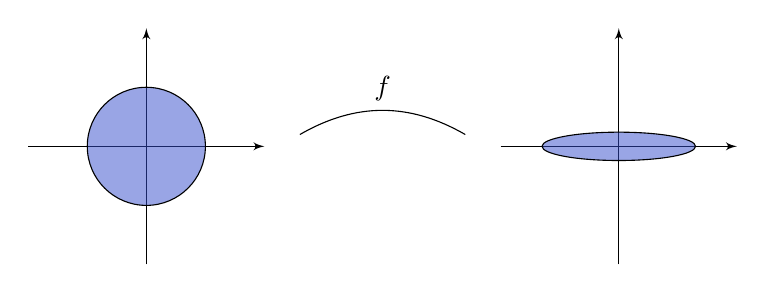
\begin{tikzpicture}[scale=1.5]
    \draw [-latex'] (-1, 0) -- (1, 0);
    \draw [-latex'] (0, -1) -- (0, 1);

    \draw [fill=mblue, fill opacity=0.5] circle [radius=0.5];

    \draw (1.3, 0.1) edge [bend left, ->] node [pos=0.5, above] {$f$} (2.7, 0.1);

    \draw [-latex'] (3, 0) -- (5, 0);
    \draw [-latex'] (4, -1) -- (4, 1);
    \draw [fill=mblue, fill opacity=0.5] (4, 0) ellipse (0.65 and 0.12);
  \end{tikzpicture}
\end{center}
By scaling it suffices to prove this for the case $r = 1$. This follows from the following result:
\begin{thm}
  If $f \in \mathcal{U}$, then $|a_2| \leq 2$.
\end{thm}
The proof of this proposition will involve quite some work. So let us just conclude the theorem from this.
\begin{proof}[Proof of Koebe-1/4 theorem]
  Suppose $f: \D \to D$ is in $\mathcal{U}$, and $z_0 \not \in D$. We shall show that $|z_0| \geq \frac{1}{4}$. Consider the function
  \[
    \tilde{f}(z) = \frac{z_0 f(z)}{z_0 - f(z)}.
  \]
  Since $\tilde{f}$ is composition of conformal transformations, it is itself conformal, and a direct computation shows $\tilde{f} \in \mathcal{U}$. Moreover, if
  \[
    f(z) = z + a_2 z^2 + \cdots,
  \]
  then
  \[
    \tilde{f}(z) = z + \left(a_2 + \frac{1}{z_0}\right)z^2 + \cdots.
  \]
  So we obtain the bounds
  \[
    |a_2|, \left|a_2 + \frac{1}{z_0}\right| \leq 2.
  \]
  By the triangle inequality, we must have $|z_0^{-1}| \leq 4$, hence $|z_0| \geq \frac{1}{4}$.
\end{proof}

The 1/4 theorem bounds the distortion in terms of the value of $f'(0)$. Conversely, if we know how much the distortion is, we can use the theorem to derive bounds on $f'(0)$.
\begin{cor}
  Let $D, \tilde{D}$ be domains and $z \in D$, $\tilde{z} \in \tilde{D}$. If $f: D \to \tilde{D}$ is a conformal transformation with $f(z) = \tilde{z}$, then
  \[
    \frac{\tilde{d}}{4d} \leq |f'(z)| \leq \frac{4\tilde{d}}{d},
  \]
  where $d = \dist(z, \partial D)$ and $\tilde{d} = \dist(\tilde{z}, \partial \tilde{D})$.
\end{cor}

\begin{proof}
  By translation, scaling and rotation, we may assume that $z = \tilde{z} = 0$, $d = 1$ and $f'(0) = 1$. Then we have
  \[
    \tilde{D} = f(D) \supseteq f(\D) \supseteq B(0, 1/4).
  \]
  So $\tilde{d} \geq \frac{1}{4}$, as desired. The other bound follows by considering $f^{-1}$.
\end{proof}
We now proceed to prove the theorem. We first obtain a bound on area, using IA Vector Calculus:
\begin{prop}
  Let $f \in \mathcal{U}$. Then
  \[
    \area(f(\D)) = \pi \sum_{n = 1}^\infty n |a_n|^2.
  \]
\end{prop}

\begin{proof}
  In the ideal world, we will have something that helps us directly compute $\area(f(\D))$. However, for the derivation to work, we need to talk about what $f$ does to the boundary of $\D$, but that is not necessarily well-defined. So we compute $\area(f(r\D))$ for $r < 1$ and then take the limit $r \to 1$.

  So fix $r \in (0, 1)$, and define the curve $\gamma(\theta) = f(re^{i\theta})$ for $\theta \in [0, 2\pi]$. Then we can compute
  \begin{align*}
    \frac{1}{2i} \int_\gamma \bar{z} \;\d z &= \frac{1}{2i} \int_\gamma (x - iy) (\d x + i\;\d y)\\
    &= \frac{1}{2i} \int_\gamma (x - iy) \;\d x + (ix + y)\;\d y\\
    &= \frac{1}{2i} \iint_{f(r\D)} 2i\;\d x\;\d y\\
    &= \area(f(r\D)),
  \end{align*}
  using Green's theorem. We can also compute the left-hand integral directly as
  \begin{align*}
    \frac{1}{2i} \int_\gamma \bar{z}\;\d z &= \frac{1}{2i} \int_0^{2\pi} \overline{f(re^{i\theta})} f'(re^{i\theta}) i re^{i\theta }\;\d \theta\\
    &= \frac{1}{2i} \int_0^{2\pi} \left(\sum_{n = 1}^\infty \bar{a}_n r^n e^{-i\theta n}\right) \left(\sum_{n = 1}^\infty a_n nr^{n - 1} e^{i\theta (n - 1)}\right) ir e^{i\theta}\;\d \theta\\
    &= \pi \sum_{n = 1}^\infty r^{2n} |a_n|^2 n.\qedhere
  \end{align*}
\end{proof}

\begin{defi}[Compact hull]\index{compact hull}
  A \emph{compact hull} is a connected compact set $K \subseteq \C$ with more than one point such that $\C \setminus K$ is connected.
\end{defi}

We want to obtain a similar area estimate for compact hulls. By the Riemann mapping theorem, if $K$ is a compact hull, then there exists a unique conformal transformation $F: \C \setminus \bar{\D}$ to $\C \setminus K$ that fixes infinity and has positive derivative at $\infty$, i.e.\ $\lim\limits_{z \to \infty} F(z)/z > 0$. Let $\mathcal{H}$ be the set of compact hulls containing $0$ with $\lim\limits_{z\to \infty} F(z)/z = 1$. If $K \in \mathcal{H}$, then the Laurent expansion of the corresponding $F$ is
\[
  F(z) = z + b_0 + \sum_{n = 1}^\infty \frac{b_n}{z^n}.
\]
Observe there is a correspondence between the space of such $F$ and $\mathcal{U}$ by sending $F$ to $1/F(1/z)$, and vice versa.
\begin{prop}
  If $K \in \mathcal{H}$, then
  \[
    \area (K) = \pi \left(1 - \sum_{n = 1}^\infty n|b_n|^2\right).
  \]
\end{prop}
Observe that the area is always non-negative. So in particular, we obtain the bound
\[
  \sum_{n = 1}^\infty n |b_n|^2 \leq 1.
\]
In particular, $|b_1| \leq 1$. This will be how we ultimately bound $|a_2|$.
\begin{proof}
  The proof is essentially the same as last time. Let $r > 1$, and let $K_r = F(r \bar{\D})$ (or, if you wish $\C \setminus F(\C \setminus r\bar{\D})$), and $\gamma(\theta) = F(r e^{i\theta})$. As in the previous proposition, we have
  \begin{align*}
    \area(K_r) &= \frac{1}{2i} \int_\gamma \bar{z} \;\d z\\
    &= \frac{1}{2i} \int_0^{2\pi} \overline{F(re^{i\theta})}F'(re^{i\theta}) ir e^{i\theta}\;\d \theta\\
    &= \pi \left(r^2 - \sum_{n = 1}^\infty n |b_n|^2 r^{-2n}\right).
  \end{align*}
  Then take the limit as $r \to 1$.
\end{proof}
By the correspondence we previously noted, this gives us some estimates on the coefficients of any $f \in \mathcal{U}$. It turns out applying this estimate directly is not good enough. Instead, we want to take the square root of $f(z^2)$.

\begin{lemma}
  Let $f \in \mathcal{U}$. Then there exists an odd function $h \in \mathcal{U}$ with $h(z)^2 = f(z^2)$.
\end{lemma}

\begin{proof}
  Note that $f(0) = 0$ by assumption, so taking the square root can potentially be problematic, since $0$ is a branch point. To get rid of the problem, define the function
  \[
    \tilde{f}(z) =
    \begin{cases}
      \frac{f(z)}{z} & z \not =0\\
      f'(0) & z = 0
    \end{cases}.
  \]
  Then $\tilde{f}$ is non-zero and conformal in $\D$, and so there is a function $g$ with $g(z)^2 = \tilde{f}(z)$. We then set
  \[
    h(z) = z g(z^2).
  \]
  Then $h$ is odd and $h^2 = z^2 g(z^2)^2 = f(z^2)$. It is also immediate that $h(0) = 0 $ and $h'(0) = 1$. We need to show $h$ is injective on $\D$. If $z_1, z_2 \in \D$ with $h(z_1) = h(z_2)$, then
  \[
    z_1 g(z_1^2) = z_2 g(z_2^2).\tag{$*$}
  \]
  By squaring, we know
  \[
    z_1^2 \tilde{f}(z_1^2) = z_2^2 \tilde{f}(z_2)^2.
  \]
  Thus, $f(z_1^2) = f(z_2^2)$ and so $z_1^2 = z_2^2$. But then $(*)$ implies $z_1 = z_2$. So $h$ is injective, and hence $h \in \mathcal{U}$.
\end{proof}

We can now prove the desired theorem.
\begin{proof}[Proof of theorem]
  We can Taylor expand
  \[
    h(z) = z + c_3 z^3 + c_5 z^5 + \cdots.
  \]
  Then comparing $h(z)^2 = f(z^2)$ implies
  \[
    c_3 = \frac{a_2}{2}.
  \]
  Setting $g(z) = \frac{1}{h(1/z)}$, we find that the $z^{-1}$ coefficient of $g$ is $-\frac{a_2}{2}$, and as we previously noted, this must be $\leq 1$.
\end{proof}
\subsection{Half-plane capacity}
\begin{defi}[Compact $\H$-hull]\index{compact $\H$-hull}
  A set $A \subseteq \H$ is called a \emph{compact $\H$-hull} if $A$ is compact, $A = \H \cap \bar{A}$ and $\H \setminus A$ is simply connected. We write $\mathcal{Q}$\index{$\mathcal{Q}$} for the collection of compact $\H$-hulls.
\end{defi}

\begin{prop}
  For each $A \in \mathcal{Q}$, there exists a unique conformal transformation $g_A: \H \setminus A \to \H$ with $|g_A(z) - a| \to 0$ as $z \to \infty$.
\end{prop}

The proof of this requires
\begin{thm}[Schwarz reflection principle]\index{Schwarz reflection principle}
  Let $D \subseteq \H$ be a simply connected domain, and let $\phi: D \to \H$ be a conformal transformation which is bounded on bounded sets and sends $\R \cap D$ to $\R$. Then $\phi$ extends by reflection to a conformal transformation on
  \[
    D^* = D \cup \{\bar{z} : z \in D\} = D \cup \bar{D}
  \]
  by setting $\phi(\bar{z}) = \overline{\phi(z)}$.\fakeqed
\end{thm}

\begin{proof}[Proof of proposition]
  The Riemann mapping theorem implies that there exists a conformal transformation $g: \H \setminus A \to \H$. Then $g(z) \to \infty$ as $z \to \infty$. By the Schwarz reflection principle, extend $g$ to a conformal transformation defined on $\C \setminus (A \cup \bar{A})$.

  By Laurent expanding $g$ at $\infty$, we can write
  \[
    g(z) = \sum_{n = -\infty}^N b_{-N} z^N.
  \]
  Since $g$ maps the real line to the real line, all $b_i$ must be real. Moreover, by injectivity, considering large $z$ shows that $N = 1$. In other words, we can write
  \[
    g(z) = b_{-1} z + b_0 + \sum_{n = 1}^\infty \frac{b_n}{z^n},
  \]
  with $b_{-1} \not= 0$. We can then define
  \[
    g_A(z) = \frac{g(z) - b_0}{b_{-1}}.
  \]
  Since $b_0$ and $b_{-1}$ are both real, this is still a conformal transformation, and $|g_A(z) - z| \to 0$ as $z \to \infty$.

  To show uniqueness, suppose $g_A, g_A'$ are two such functions. Then $g_A' \circ g_A^{-1}: \H \to \H$ is such a function for $A = \emptyset$. Thus, it suffices to show that if $g: \H \to \H$ is a conformal mapping such that $g(z) - z \to 0$ as $z \to \infty$, then in fact $g = z$. But we can expand $g(z) - z$ as
  \[
    g(z) - z = \sum_{n = 1}^\infty \frac{c_n}{z^n},
  \]
  and this has to be holomorphic at $0$. So $c_n = 0$ for all $n$, and we are done.
\end{proof}

\begin{defi}[Half-plane capacity]\index{half-plane capacity}
  Let $A \in \mathcal{Q}$. Then the \emph{half-plane capacity} of $A$ is defined to be
  \[
    \hcap(A) = \lim_{z \to \infty} z(g_A(z) - z).
  \]
  Thus, we have
  \[
    g_A(z) = z + \frac{\hcap(A)}{z} + \sum_{n = 2}^\infty \frac{b_n}{z^n}.
  \]
\end{defi}
We shall show that $\hcap(A)$ is in fact non-negative and increasing.

\begin{eg}
  $z \mapsto \sqrt{z^2 + 4t}$ is the unique conformal transformation $\H \setminus [0, \sqrt{t}i] \to \H$ with $|\sqrt{z^2 + 4z} - z| \to 0$ as $z \to \infty$. We can expand
  \[
    \sqrt{z^2 + 4t} = z + \frac{2t}{z} + \cdots.
  \]
  Thus, we know that $\hcap([0, 2\sqrt{t} i]) = 2t$.
\end{eg}

\begin{eg}
  The map $z \mapsto z + \frac{1}{z}$ maps $\H \setminus \bar{\D} \to \H$. Again, we have $|z + \frac{1}{z} - z| \to 0$ as $z \to \infty$, and so $\hcap(\H \cap \bar{D}) = 1$.
\end{eg}
We note some immediate properties:
\begin{prop}\leavevmode
  \begin{enumerate}
    \item Scaling: If $r > 0$ and $A \in \mathcal{Q}$, then $\hcap(rA) = r^2 \hcap(A)$.
    \item Translation invariance: If $x \in \R$ and $a \in \mathcal{Q}$, then $\hcap(A + x) = \hcap(A)$.
    \item Monotonicity: If $A, \tilde{A} \in \mathcal{Q}$ are such that $A \subseteq \tilde{A}$. Then $\hcap(A) \leq \hcap(\tilde{A})$.
  \end{enumerate}
\end{prop}

\begin{proof}\leavevmode
  \begin{enumerate}
    \item We have $g_{rA}(z) = r g_A(z/r)$.
    \item Observe $g_{A + x}(z) = g_A(z - x) + x$.
    \item We can write
      \[
        g_{\tilde{A}} = g_{g_A(\tilde{A} \setminus A)} \circ g_A.
      \]
      Thus, expanding out tells us
      \[
        \hcap(\tilde{A}) = \hcap(A) + \hcap(g_A(\tilde{A}\setminus A)).
      \]
      So the desired result follows if we know that the half-plane capacity is non-negative, which we will prove next.\qedhere
  \end{enumerate}
\end{proof}
Observe that these results together imply that if $A \in \mathcal{Q}$ and $A \subseteq r(\bar{\D} \cap \H)$, then
\[
  \hcap(A) \leq \hcap(r(\bar{\D} \cap \H)) \leq r^2 \hcap (\bar{\D} \cap \H) = r^2.
\]
So we know that $\hcap(A) \leq 4 \diam(A)^2$

How can we prove non-negativity? After a long time, probability theory is going to re-enter the course, because we are going to use Brownian motion to prove this!

\begin{prop}
  Suppose $A \in \mathcal{Q}$ and $B_t$ be complex Brownian motion, and $\tau = \inf\{t \geq 0: B_t \not \in \H \setminus A\}$. Then
  \begin{enumerate}
    \item For all $z \in \H \setminus A$, we have $\im(z - g_A(z)) = \E_z[\im(B_\tau)]$
    \item
      \[
        \hcap(A) = \lim_{y \to \infty} y \E_y[\im(B_\tau)].
      \]
    \item If $A \subseteq \bar{\D} \cap \H$, then
      \[
        \hcap(A) = \frac{2}{\pi} \int_0^\pi \E_{e^{i\theta}}[\im(B_\tau)]\sin \theta \;\d \theta.
      \]
  \end{enumerate}
\end{prop}
It is immediate from (ii) that
\begin{cor}
  $\hcap(A) \geq 0$.
\end{cor}

\begin{proof}\leavevmode
  \begin{enumerate}
    \item Let $\phi(z) = \im(z - g_A(z))$. Then $\phi$ is harmonic on $\H \setminus A$, since $z - g_A(z)$ is holomorphic. As
      \[
        g_A(Z) = z + \frac{\hcap (A)}{z} + \cdots
      \]
      and $\im(g_A(z)) = 0$ when $z \in \partial(\H \setminus A)$, we know $\varphi$ is harmonic, continuous and bounded. These are exactly the conditions needed to solve the Dirichlet problem using Brownian motion. So the result follows.

    \item We have
      \begin{align*}
        \hcap(A) &= \lim_{z \to \infty} z (g_A(z) - z) \\
        &= \lim_{y \to \infty} (iy) (g_A(iy) - iy)\\
        &= \lim_{y \to \infty} y \im (iy - g_A(iy))\\
        &= \lim_{y \to \infty} y \E_{iy} [\im(B_\tau)]
      \end{align*}
      where we use the fact that $\hcap(A)$ is real, so we can take the limit of the real part instead.
    \item See example sheet.\qedhere
  \end{enumerate}
\end{proof}

In some sense, what we used above is that Brownian motion is conformally invariant, where we used a conformal mapping to transfer between our knowledge of Brownian motion on $\H$ to that on $\H \setminus \D$. Informally, this says the conformal image of a Brownian motion is a Brownian motion, up to a (random) change of time, and in particular, the image of the path is unchanged.

We have in fact seen this before. We have seen that rotations preserve Brownian motion, and so does scaling, except when we scale we need to scale our time as well. Since conformal mappings are locally rotations and scalings, the result should not be surprising. The random time change happens because we are performing different transformations all over the domain.

\begin{thm}
  Let $D, \tilde{D} \subseteq \C$ be domains, and $f: D \to \tilde{D}$ a conformal transformation. Let $B, \tilde{B}$ be Brownian motions starting from $z \in D, \tilde{z} \in \tilde{D}$ respectively, with $f(z) = \tilde{z}$. Let
  \begin{align*}
    \tau = \inf\{t \geq 0: B_t \not \in D\}\\
    \tilde{\tau} = \inf\{t \geq 0: \tilde{B}_t \not \in \tilde{D}\}
  \end{align*}
  Set
  \begin{align*}
    \tau' &= \int_0^\tau |f'(B_s)|^2\;\d s\\
    \sigma(t) &= \inf\left\{s \geq 0 : \int_0^s |f'(B_r)|^2\;\d r = t\right\}\\
    B_t' = f(B_{\sigma(t)}).
  \end{align*}
  Then $(B_t' : t < \tilde{\tau}')$ has the same distribution as $(\tilde{B}_t: t < \tilde{\tau})$.
\end{thm}

\begin{proof}
  See Stochastic Calculus.
\end{proof}

\begin{eg}
  We can use conformal invariance to deduce the first exist distribution of a Brownian motion from different domains. First of all, observe that from $\D$, starting from the origin, the first exit distribution is uniform. Thus, applying a conformal transformation, we see that the exit distribution starting from $z$ is
  \[
    f(e^{i\theta}) = \frac{1}{2\pi}\left(\frac{1 - |z|^2}{ |e^{i\theta} - z|}\right).
  \]
  Similarly, on $\H$, starting from $z = x + iy$, the exit distribution is
  \[
    f(u) = \frac{1}{\pi} \frac{y}{(x - u)^2 + y^2}.
  \]
  Note that if $x = 0, y = 1$, then this is just
  \[
    f(u) \frac{1}{\pi}\left(\frac{1}{u^2 + 1}\right).
  \]
  This is the Cauchy distribution!
\end{eg}

\section{Loewner's theorem}
In this chapter, we shall prove Loewner's theorem.
\subsection{Key estimates}
We first prove some estimates needed in Loewner's theorem.
\begin{prop}
  Suppose $A \in \mathcal{Q}$, and $B$ is a complex Brownian motion, and
  \[
    \tau = \inf \{t \geq 0: B_t \not \in \H \setminus A\}.
  \]
  Then
  \begin{itemize}
    \item If $x > \rad(A)$, then
      \[
        g_A(x) = \lim_{y \to \infty} \pi y \left(\frac{1}{2} + \P_{iy} [B_\tau \in [x, \infty)]\right).
      \]
    \item If $x < -\rad(A)$, then
      \[
        g_A(x) = \lim_{y \to \infty} \pi y \left(\frac{1}{2} - \P_{iy}[B_\tau \in (-\infty, x]]\right).
      \]
  \end{itemize}
\end{prop}

\begin{proof}
  Suppose $A = \emptyset$. Then
  \begin{align*}
    &\hphantom{{}={}}\lim_{y \to \infty} \pi y \left(\frac{1}{2} \P_{iy}[B_\tau \in [x, \infty)]\right)\\
    &= \lim_{y \to \infty} \P_{iy} [B_\tau \in [0, x)]\\
    &=\lim_{y \to \infty} \pi y \int_0^x \frac{y}{\pi (s^2 + y^2)}\;\d s\\
    &= x,
  \end{align*}
  where the first equality follows from the fact that Brownian motion exits through the positive reals with probability $\frac{1}{2}$, and the second equality is an exercise on the first example sheet.

  Now suppose $A \not= \emptyset$. We will use conformal invariance to reduce this to the case above. We write $g_A = u_A + i v_A$. We let
  \[
    \sigma = \inf \{t > 0: B_t \not \in \H\}.
  \]
  Then we know
  \begin{align*}
    \P_{iy} [B_\tau \in [x, \infty)] &= \P_{g_A(iy)} [B_\sigma \in [g_A(x), \infty)]\\
    &= \P_{iv_A(iy)} [B_\sigma \in [g_A(x) - u_A(iy), \infty)].
  \end{align*}
  Since $g_A(z) - z \to 0$ as $z \to \infty$, it follows that $\frac{v_A(iy)}{y} \to 1$ and $y u_A(iy) \to 0$ as $y \to \infty$. So we have
  \[
    \left|\P_{iv_A(iy)} [B_\sigma \in [g_A(x) - u_A(iy), \infty)] - \P_{iy}[B_\sigma \in g_A(x), \infty)]\right| = o(y^{-1}\text{ as }y \to \infty.
  \]
  Combining with the case $A = \emptyset$, the the proposition follows.
\end{proof}

\begin{cor}
  If $A \in \mathcal{Q}$, $\rad(A) \leq 1$, then
  \begin{align*}
    x &\leq g_A(x) \leq x + \frac{1}{x}&&\text{if }x > 1\\
    x + \frac{1}{x} &\leq g_A(x) \leq x && \text{if }x < -1.
  \end{align*}
  Here recall that $z \mapsto z + \frac{1}{z}$ sends $\H \setminus \bar{\D}$ to $\H$. Moreover, for all $A \in \mathcal{Q}$, we have
  \[
    |g_A(z) - z| \leq 3 \rad(A).
  \]
\end{cor}

\begin{proof}
  Exercise on the first example sheet.
\end{proof}
This corollary gives us a ``zeroth order'' bound on $g_A(z) - z$. We can obtain a better first-order bound as follows:
\begin{prop}
  There is a constant $c > 0$ so that for every $A \in \mathcal{Q}$ and $|z| > 2 \rad(A)$, we have
  \[
    \left|g_a(z) - \left(z + \frac{\hcap(A)}{z}\right)\right| \leq \frac{c - \rad(A) \cdot \hcap(A)}{|z|^2}.
  \]
\end{prop}

\begin{proof}
  Performing a scaling if necessary, we can assume that $\rad(A) = 1$. Let
  \[
    h(z) = z + \frac{\hcap (A)}{z} - g_A(z).
  \]
  We aim to control the imaginary part of this, and then use the Cauchy--Riemann equations to control the real part as well. We let
  \[
    v(z) = \im(h(z)) = \im(z - g_A(z)) = \frac{\im (z)}{|z|^2} \hcap(A).
  \]
  Let $B$ be a complex Brownian motion, and let
  \begin{align*}
    \sigma &= \inf \{t \geq 0: B_t \not \in \H \setminus \bar{\D}\}\\
    \tau &= \inf \{t \geq 0: B_t \not \in \H\}.
  \end{align*}
  Let $p(z, e^{i\theta})$ be the density with respect to the Lebesgue measure at $e^{i\theta}$ for $B_\sigma$. Then
  \[
    \im(z - g_A(z)) = \int_0^\pi \E_{e^{i\theta}} [\im(B_\tau)] p(z, e^{i\theta})\;\d \theta
  \]
  by the strong Markov property at the time $\sigma$. In the first example sheet Q3, we show that
  \[
    p(z, e^{i\theta}) = \frac{2}{\pi} \frac{\im(z)}{|z|^2} \sin \theta \left(1 + O\left(\frac{1}{|z|}\right)\right).\tag{$*$}
  \]
  We also have
  \[
    \hcap(A) = \frac{2}{\pi} \int_0^\pi \E_{e^{i\theta}} [\im(B_\tau)] \sin \theta \;\d \theta.
  \]
  So
  \begin{align*}
    |v(z)| &= \left| \im (z - g_A(z)) - \frac{\im(z)}{|z|^2} \hcap(A)\right|\\
    &= \left| \int_0^\pi \E_{e^{i\theta}} [\im(B_\tau)] p(z, e^{i\theta})\;\d \theta - \frac{\im(z)}{|z|^2} \cdot \frac{2}{\pi} \int_0^\pi \E_{e^{i\theta}}[\im(B_\tau)] \sin \theta \;\d \theta\right|.
  \end{align*}
  By applying $(*)$, we get
  \[
    |v(z)| \leq c \frac{c \hcap (A) \im(z)}{|z|^3}.
  \]
  where $c$ is a constant.

  Recall that $v$ is harmonic as it is the imaginary part of a holomorphic function. By example sheet 1 Q9, we have
  \[
    |\partial_x v(z)| \leq \frac{c \hcap(A)}{|z|^3},\quad |\partial_y v(z)| \leq \frac{c \hcap(A)}{|z|^3}.
  \]
  By the Cauchy--Riemann equations, $\re(h(z))$ satsifies the same bounds. So we know that
  \[
    |h'(z)| \leq \frac{c \hcap(A)}{|z|^3}.
  \]
  Then
  \[
    h(iy) = \int_y^\infty h'(is)\;\d s,
  \]
  since $h(iy) \to 0$ as $y \to \infty$. Taking absolute values, we have
  \begin{align*}
    |h(iy) &= \int_y^\infty |h'(is)|\;\d s\\
    &\leq c \hcap (A) \int_y^\infty s^{-3} \;\d s\\
    &\leq c' \hcap(A) y^{-z}.
  \end{align*}
  To get the desired bound for a general $z$, integrate $h'$ along the boundary of the circle of radius $|z|$ to get
  \[
    |h(z)| = |h(r e^{i\theta})| \leq \frac{c \hcap(A)}{|z|^2} + h(iz).\qedhere
  \]
\end{proof}

The following is a very useful fact about Brownian motion:
\begin{thm}[Beurling estimate]\index{Beurling estimate}
  There exists a constant $c > 0$ so that the following holds. Let $B$ be a complex Brownian motion, and $A \subseteq \bar{\D}$ be connected, $0 \in A$, ,and $A \cap \partial \bar{\D} \not= \emptyset$. Then for $z \in \D$, we have
  \[
    \P_z[B[0, \tau] \cap A = \emptyset] \leq c |z|^{1/2},
  \]
  where $\tau = \inf \{t \geq 0: B_t \not \in \D\}$.
\end{thm}
In the Beurling estimate, the worst case behaviour is obtained when $A = [-i, 0]$.

We will not prove this, since it is quite tricky to prove.

To prove one more theorem, we need one more estimate, which uses the Beurling estimate.

\begin{prop}
  There exists a constant $c > 0$ so that the following is true: Suppose $A, \tilde{A} \in \mathcal{Q}$ with $A \subseteq \tilde{A}$ and $\tilde{A} \setminus A$ is coonnected. Then
  \[
    \diam(g_A(\tilde{A}\setminus A))\leq c
    \begin{cases}
      (dr)^{1/2} & d \leq r\\
      \rad(\tilde{A}) & d > r
    \end{cases},
  \]
  where
  \[
    d = \diam(\tilde{A} \setminus A),\quad r = \sup \{\im (z) : z \in \tilde{A}\}.
  \]
\end{prop}

\begin{proof}
  By scaling, we can assume that $r = 1$.
  \begin{itemize}
    \item If $d \geq 1$, then the result follows since
      \[
        |g_A(z) - z| \leq 3 \rad(A),
      \]
      and so
      \[
        \diam(g_A(\tilde{A}\setminus A)) \leq \diam(A) + 6 \rad(A) \leq 8 \diam(\tilde{A}).
      \]
    \item If $d < 1$, fix $z \in \H$ so that $U = B(z, d) \supseteq \tilde{A} \setminus A$. It then suffices to bound the size of $g_A(U)$ (or, to be precise, $g_A(U \setminus A)$).

      Let $B$ be a complex Brownian motion starting from $iy$ with $y \geq 2$. Let
      \[
        \tau = \inf \{t \geq 0: B_t \not \in \H \setminus A\}.
      \]
      For $B[0, \tau]$ to reach $U$, it must
      \begin{enumerate}
        \item Reach $B(z, 1)$ without leaving $\H \setminus A$, which occurs with probability at most $c/y$ for some constant $c$, by example sheet.
        \item It must then hit $U$ before leaving $\H \setminus A$. By the Beurling estimate, this occurs with probability $\leq c d^{1/2}$.
      \end{enumerate}
      Combining the two, we see that
      \[
        \limsup_{y \to \infty} \P_{iy}[B[0, \tau] \cap U \not= \emptyset] \leq c d^{1/2}.
      \]
      By the conformal invariance of Brownian motion, if $\sigma = \inf \{t \geq 0 : B_t \not \in \H\}$, this implies
      \[
        \limsup_{y \to \infty} y \P_y [B[0, \sigma] \cap g_A(\tilde{A} \setminus A) \not= \emptyset] \leq c d^{1/2}.
      \]
      Since $g_A(\tilde{A} \setminus A)$ is connected, by Q10 of example sheet 1, we have
      \[
        \diam(g_A(\tilde{A} \setminus A)) \leq cd^{1/2}.\qedhere
      \]%\qedhere
  \end{itemize}
\end{proof}

\begin{defi}
  Suppose $(A_t)_{t \geq 0}$ is a family of compact $\H$-hulls. We say that $(A_t)$ is
  \begin{enumerate}
    \item \term{non-decreasing} if $s \leq t$ implies $A_s \subseteq A_t$.
    \item \term{locally growning} if for all $Y > 0$ and $\varepsilon > 0$, there exists $\delta > 0$ such that $0 \leq s \leq t \leq s + \delta \leq T$. So
      \[
        \diam(g_{A_s}(A_t \setminus A_s)) \leq \varepsilon.
      \]
      This is a continuity condition.
    \item \term{parametrized by half-plane capacity} if $\hcap(A_t) = 2t$ for all $t \geq 0$.
  \end{enumerate}
  We write $\mathcal{A}$ be the set of families of compact $\H$-hulls which satisfy (i) to (iii). We write $\mathcal{A}_T$ for the set of such families defined on $[0, T]$.
\end{defi}

\begin{eg}
  If $\gamma$ is is a simple curve in $\H$ starting from $0$ and $A_t = \gamma[0, t]$. This clearly satisfies (i), and the previous proposition tells us this satsifies (ii). On the first example sheet, we show that we can reparametrize $\gamma$ so that $\hcap(A_t) = 2t$ for all $t \geq 0$. Upon doing so, we have $A_t \in \mathcal{A}$.
\end{eg}

\begin{thm} % Loewner's theorem.
  Suppose that $(A_t) \in \mathcal{A}$. Let $g_t = g_{A_t}$. Then there exists a continuous function $U: [0, \infty) \to \R$ so that
  \[
    \partial_t g_t (z) = \frac{z}{g_t(z) - U_t},\quad g_0(z) = z.
  \]
\end{thm}
THis is known as the \term{chordal Loewner ODE}, and $U$ is called the \term{driving function}.

\begin{proof}
  Note that $\bigcap_{s \geq t} g_t(A_s)$ contains a single point, as the hulls are locally growing. Call this point $U_t$. Using the local growth property, it is not hard to see that $U_t$ is continuous in $t$.

  Recall that if $A \in \mathcal{Q}$, then
  \[
    g_A(z) = z + \frac{\hcap(A)}{z} + O\left(\frac{\hcap(A) \rad(A)}{|z|^2}\right).
  \]
  If $x \in \R$, then as $g_{A + x}(z) - x = g_A(z - x)$, we have
  \[
    g_A(z) = g_A(z + x) - x = z + \frac{\hcap(z)}{z + x} + O\left(\frac{\hcap(A) \rad(A + x)}{|z + x|^2}\right).\tag{$*$}
  \]
  Fix $\varepsilon > 0$. For $0 \leq s \leq t$, let
  \[
    g_{s, t} = g_t \circ g_s^{-1}.
  \]
  Note that
  \[
    \hcap(g_T(A_{t + \varepsilon} \setminus A_t)) = 2 \varepsilon.
  \]
  Apply $(*)$ with $A = g_t(A_{t + \varepsilon} \setminus A_t)$, $x = -U_t$, and use that $\rad(A + x) = \rad(A - U_t) \leq \diam(A)$ to see that
  \[
    g_A(z) = g_{t, t + \varepsilon}(z) = z + \frac{2\varepsilon}{z - U_t} + 2 \varepsilon \diam(g_t(A_{t + \varepsilon} \setminus A_t))O\left(\frac{1}{|z - U_t|^2}\right).
  \]
  So
  \begin{align*}
    g_{t + \varepsilon}(z) - g(t)z &= (g_{t, t + \varepsilon} - g_{t, t}) \circ g_t(z)\\
    &= \frac{2\varepsilon}{g_t(z) - U_t} + 2\varepsilon \diam(g_t(A_{t + \varepsilon} \setminus A_t)) O\left(\frac{1}{|g_t(z) - U_t|^2}\right).
  \end{align*}
  Dividing both sides by $\varepsilon$ and taking the limit as $\varepsilon \to 0$, the desired result follows since $\diam(g_t(A_{t + \varepsilon} \setminus A_t)) \to 0$.
\end{proof}

We can ask about the reverse procedure --- given a continuous function $U_t$, can we find a collection $A_t \in \mathcal{A}$ whose driving function is $U_t$? We can simply let $g_t$ be the solution to this differential equation. We can then let
\[
  A_t = \H \setminus \mathrm{domain}(g_t),
\]
and then this is a family in $\mathcal{A}$, which is an exercise on the example sheet.

\section{Schramm--Loewner evolution}
SLE is what we get when we pick $U_t$ to be a random function, so that we get a random family of hulls.

Suppose $(A_t)$ is a \emph{random} family in $\mathcal{A}$, encoded by $U$. Let $\mathcal{F}_t = \sigma(U_s: s \leq t)$.
\begin{defi}[Conformal Markov property]\index{conformal Markov property}
  We say that $(A_t)$ satisfy the \emph{conformal Markov property} if
  \begin{enumerate}
    \item Given $\mathcal{F}_t$, $(g_t(A_{t + s}) - U_t)_{s \geq 0} \overset{d}{=} (A_s)_{s \geq 0}$.
    \item Scale-invariance: $(r A_{t/r^2} )_{t \geq 0} \overset{d}{=} (A_t)$.
  \end{enumerate}
\end{defi}
Here (i) is the Markov property, and the second part is the conformal part, since the only conformal maps $\H \to \H$ that fix $0$ and $\infty$ are the rescalings.

\begin{thm}[Schramm]
  If $(A_t)$ satisfy the conformal Markov property, then there exists $\kappa \geq 0$ so that $U_t = \sqrt{\kappa} B_t$, where $B$ is a standard Brownian motion.
\end{thm}

\begin{prop}
  The first property is exactly the same thing as saying that $\mathcal{F}_t$, we have
  \[
    (U_{t + s} - U_t)_{s \geq 0} \overset{d}{=} (U_s).
  \]
  So $U_t$ is a continuous process with stationary, independent increments. This implies there exists $\kappa \geq 0$ and $a \in \R$ such that
  \[
    U_t = \sqrt{\kappa}B_t + at,
  \]
  where $B$ is a standard Brownian motion. Then the second part says
  \[
    (r U_{t/r^2})_{t \geq 0} \overset{d}{=} (U_t)_{t \geq 0}.
  \]
  So $U$ satisfies Brownian scaling. Plugging this in, we know
  \[
    r \sqrt{\kappa} B_{t/r^2} + at/r \overset{d}{=} r \sqrt{\kappa} B_t + at.
  \]
  Since $r \sqrt{\kappa} B_{t/r^2} \overset{d}{=} r \sqrt{\kappa} B_t$, we must have $a = 0$.
\end{prop}

This finally gives us the definition of SLE.
\begin{defi}[Schramm--Loewner evolution]\index{Schramm--Loewner evolution}\index{SLE}
  For $\kappa > 0$, $\SLE_\kappa$ is the random family of hulls encoded by $U_t = \sqrt{\kappa} B_t$, where $B$ is a standard Brownian motion.
\end{defi}
When $\kappa = 0$, we have $U_t = 0$. This corresponds to the curve $\gamma(t) = 2 \sqrt{t} i$.

It turns out that $\SLE_\kappa$ is ``generated'' by a continuous curve $\eta$. This means that $\H \setminus A_t$ is the unbounded component of $\H \setminus \eta([0, t])$ for all $t \geq 0$. We will assume this fact. It was first proved by Rhode--Schramm in 2005.

The behaviour strongly depends on $\kappa$. We will see that if $\kappa \leq 4$, then this is a simple curve; if $\kappa \in (4, 8)$, then it is self-intersecting; if $\kappa \geq 8$, then it is space-filling.

SLE is singled out by the conformal Markov property. This comes from conjectures made in the physics literature about scaling limits of discrete lattice models (percolation, loop-erased random walks, Ising model, etc.). People believed for a long time that if we take the scaling limit of such evolutions, then we get something that is conformal invariant, and so they are SLEs.

An important tool for dealing with SLEs is via stochastic calculus, since it is defined by a differential equation where we put in a Brownian motion.

\section{Review of stochastic calculus}
In stochastic calculus, the basic object is continuous semi-martingales. We set
\[
  X_t = M_t + A_t,
\]
where $M$ is a continuous local martingale and $A$ is continuous with bounded variation.

Important concepts in stochastic calculus include
\begin{enumerate}
  \item Stochastic integrals
  \item Quadratic variation
  \item It\^o's formula
  \item L\'evy characterization of Brownian motion
  \item Stochastic differential equations
\end{enumerate}

The general setting is that we have a probability space $(\Omega, \mathcal{F}, \P)$ with a continuous time filtration $\mathcal{F}_t$, which satisfies the ``usual conditions'', namely $\mathcal{F}_0$ contains all $\P$-null sets, and $\mathcal{F}_t$ is right continuous, i.e.
\[
  \mathcal{F}_t = \bigcap_{s > t} \mathcal{F}_s.
\]
\subsubsection*{Stochastic integral}
If $X_t = M_t + A_t$ is a continuous semi-martingale, and $H_t$ is a previsible process, we set
\[
  \int_0^t H_s \;\d X_s = \int_0^t H_s \;\d M_s + \int_0^t H_s \;\d A_s,
\]
where the first integral is the It\^o integral, which gives a continuous local martingale, and the second integral is the Lebesgue--Stieltjes integral, and gives a continuous bounded variation process.

The It\^o integral is defined in the same spirit as the Riemann integral. The key thing that makes it work is that there is ``extra cancellation'' in the definition, from the fact that we are integrating against a martingale, and so makes the integral converge even though the process we are integrating against is not of bounded variation.
\subsubsection*{Quadratic variation}
If $M$ is a continuous local martingale, then the quadratic variation is
\[
  [M]_t = \lim_{n \to \infty} \sum_{k = 0}^{\lceil 2^n t\rceil - 1}(M_{(k + 1)2^{-n}} - M_{k2^{-n}})^2,
\]
and is the unique continuous non-decreasing process of bounded variation such that $M_t^2 - [M]_t$ is a continuous local martingale. The quadratic variation of a bounded variation process is always zero. So if $X$ is a semi-martingale, then we define
\[
  [X]_t = [M + A]_t = [M]_t.
\]
Also, we have
\[
  \left[\int_0^{(\ph)} H_s\;\d M_s\right]_t = \int_0^t H_s^2 \;\d [M]_s,
\]
where the integral on the right is the Lebesgue--Stieltjes integral.

\subsubsection*{It\^o's formula}
It\^o's formula is the stochastic calculus' analogue of the fundamental theorem of calculus. It takes a bit of work to prove It\^o's formula, but it is easy to understand what the intuition is. If $f \in C^2$, then we have
\[
  f(t) = f(0) + \sum_{k = 1}^n (f(t_k) - f(t_{k - 1}))
\]
for any partition $0 = t_0 < \cdots < t_n = t$. If we were to do a regular fundamental theorem of calculus, then we can perform a Taylor approximation
\[
  f(t) = f(0) = \sum_{k = 1}^n f'(t_{k - 1})((t_k - t_{k - 1}) + o(t_k - t_{k - 1})) \to f(0) + \int_0^t f'(s)\;\d s
\]
as $\max |t_k - t_{k - 1}| \to 0$.

In It\^o's formula, we want to do the same thing but with Brownian motion. Suppose $B$ is a Brownian motion. Then
\[
  f(B_t) = f(B_0) = \sum_{k = 1}^n (f(B_{t_k}) - f(B_{t_{k - 1}})).
\]
When we do a Taylor expansion of this, we have to be a bit more careful than before, as we cannot ignore all the higher order terms. The point is that the quadratic variation of $B_t$ is non-zero. We write this as
\[
  f(0) + \sum_{k = 1}^n \Big[f'(B_{t_{k\!-\!1}}) (B_{t_k} - B_{t_{k\!-\!1}}) + \frac{1}{2} f''(B_{t_{k\!-\!1}}) (B_{t_k} - B_{t_{k\!-\!1}})^2 + o((B_{t_k} + B_{t_{k\!-\!1}})^2)\Big].
\]
Taking the limit, and using that $\E[(B_{t_k} - B_{t_{k - 1}})^2] = t_k - t_{k - 1}$, we get
\[
  f(B_t) = f(0) \int_0^t f'(B_s)\;\d B_s + \frac{1}{2} \int_0^t f''(B_s) \;\d s.
\]
More generally, if $X_t = M_t + A_t$ is a continuous semi-martingale, and $f \in C^{1, 2}(\R_t \times \R)$, so that it is $C^1$ in the first variable and $C^2$ in the second, then
\begin{multline*}
  f(t, X_t) = f(0, X_0) + \int_0^t \partial_s f(s, X_s) \;\d s + \int_0^t \partial_x f(s, X)\;\d A_s\\
  + \frac{1}{2} \int_0^t \partial_x^2 f(s, X_s) \;\d [M]_s + \int_0^t \partial_x f(s, X_s) \;\d M_s.
\end{multline*}

\subsubsection*{L\'evy characterization of Brownian motion}
\begin{thm}[L\'evy characterization]\index{L\'evy characterization}
  Let $M_t$ is a continuous local martingale with $[M]_t = t$ for $t \geq 0$, then $M_t$ is a standard Brownian motion.
\end{thm}

\begin{proof}[Proof sketch]
  Use It\^o's formula with the exponential moment generating function $e^{i\theta M_t + \theta^2/2 [M]_t}$.
\end{proof}

\subsubsection*{Stochastic differential equations}
Suppose $(\Omega, \mathcal{F}, \P)$ and $(\mathcal{F}_t)$ are as before, and $(B_t)$ is a Brownian motion adapted to $(\mathcal{F}_t)$. We say a process $X_t$ satisfies satisfies the \term{stochastic differential equation}
\[
  \d X_t = b(X_t) \;\d t + \sigma(X_t) \;\d B_t
\]
for functions $b, \sigma$ iff
\[
  X_t = \int_0^t b(X_s) \;\d s + \int_0^t \sigma(X_s) \;\d B_s + X_0
\]
for all $t \geq 0$. At the end of the stochastic calculus course, we will see that there is a unique solution to this equation provided $b, \sigma$ are Lipschitz functions.

This in particular implies we can solve
\[
  \partial_t g_t(z) = \frac{2}{g_t(z) - U_t},\quad g_0(z) = z
\]
for $U_t = \sqrt{\kappa} B_t$, where $B_t$ is a standard Brownian motion.

\section{Phases of SLE}
Last time, we made some claims about the behaviour of $\SLE_\kappa$ for different values of $\kappa$. To do this, we need to understand Bessel processes.

\subsection{Bessel processes}
Suppose $X = (B^1, \ldots, B^d)$ is a $d$-dimensional standard Brownian motion. Let
\[
  Z_t = \|X_t\|^2 = (B_t^1)^2 + (B_t^2)^2 + \cdots + (B_t^d)^2.
\]
It\^o's formula implies
\[
  Z_t = Z_0 + 2 \int_0^t B_s^1 \;\d B_s^1 + \cdots + 2 \int_0^t B_s^d\;\d B_s^d + d\cdot t.
\]
Set
\[
  Y_t = \int_0^t \frac{B_s^1 \;\d B_s^1 + \cdots + B_s^d \;\d B_s^d}{Z_s^{1/2}}.
\]
Then we have
\[
  Z_t = Z_0 = 2 \int_0^t Z_s^{1/2} \;\d Y_s + d\cdot t.
\]
What do we know about $Y_t$? This is a continuous local martingale. The quadratic variation is then equal to
\[
  [Y]_t = \int_0^t \frac{(B_s^1)^2 + \cdots + (B_s^d)^2}{Z_s}\;\d s = t.
\]
By the L\'evy characterization, $Y_T$ is a standard Brownian motion. So we can write
\[
  Z_t = Z_0 + 2 \int_0^t Z_s^{1/2}\;\d \tilde{B}_s + dt,
\]
where $\tilde{B}$ is a standard Brownian motion. The differential form of this equation is the
\[
  \d Z_t = 2 Z_t^{1/2} \;\d \tilde{B}_t + d \cdot \d t.
\]
This is called the \term{square Bessel stochastic differential equation} with dimension $d$. We say $Z_t$ is a \term{square Bessel process} (\term{BESQ}) with dimension $d$.

We apply It\^o's formula again with $f(x) = x^{1/2}$, to get
\begin{align*}
  Z_t^{1/2} &= Z_0^{1/2} + \frac{1}{2} \int_0^t Z_s^{-1/2} \;\d Z_s - \frac{1}{8} \int_0^t Z_s^{-3/2} \;\d [Z]_s\\
  &= Z_0^{1/2} + \tilde{B}_t + \frac{d}{2} \int_0^t Z_s^{-1/2}\;\d s - \frac{1}{2} \int_0^t Z_s^{-1/2} \;\d s\\
  &= Z_0^{1/2} + \frac{d - 1}{2} \int_0^t Z_s^{-1/2}\;\d s + \tilde{B}_t.
\end{align*}
Setting $U_t = Z_t^{1/2}$, we have
\[
  U_t = U_0 + \frac{d - 1}{2} \int_0^t U_s^{-1}\;\d s + \tilde{B}_t.
\]
The differential form of this equation is then
\[
  \d U_t = \left(\frac{d - 1}{2}\right) U_t^{-1}\;\d t + \d \tilde{B}_t.
\]
This is the \term{Bessel stochastic differential equation} of dimension $d$, and we set $U_t$ is a \term{Bessel process} of dimension $d$ (\term{BES\textsuperscript{$d$}}). This tells us how the modulus of a standard Brownian motion evolves.

But, the BES$^d$ has a solution for all $d \in \R$. The only problem with solving this stochastic differential equation is that $U_t^{-1}$ is not a Lipschitz function as $U_t \to 0$. To avoid this problem, we say this is defined up to when it hits $0$.

\begin{prop}
  Let $d \in \R$, and $U_t$ a BES$^d$.
  \begin{enumerate}
    \item If $d < 2$, then $U_t$ hits $0$ almost surely.
    \item If $d \geq 2$, then $U_t$ doesn't hit $0$ almost surely.
  \end{enumerate}
\end{prop}
This agrees with what we expect from the recurrence of Brownian motion, for integral $d$. In particular, for $d = 2$, a Brownian motion gets arbitrarily close to $0$ infinitely often, so we expect that if we are just a bit lower than $d = 2$, we would hit $0$ almost surely.
\begin{proof}
  Consider the process $U_t^{2 - d}$. By It\^o's formula, we have
  \begin{align*}
    U_t^{2 - d} &= U_0^{2 - d} + \int_0^t (2 - d) U_s^{1 - d} \;\d U_s + \frac{1}{2} \int_0^t (2 - d) (1 - d) U_s^{-d} \;\d [U]_s\\
    &= U_0^{2 - d} + \int_0^t (2 - d) U_s^{1 - d} \;\d \tilde{B}_t + \int_0^t \frac{(2 - d)(d - 1)}{2 U_s} U_s^{1 - d}\;\d s \\
    &\hphantom{aaaaaaaaa}+ \frac{1}{2} \int_0^t (2 - d)(1 - d) U_s^{-d}\;\d s\\
    &= U_0^{2 - d} + \int_0^t (2 - d) U_s^{1 - d}\;\d \tilde{B}_s.
  \end{align*}
  Therefore $U_t$ is a continuous local martingale.

  Now for $a \in \R$, let
  \[
    \tau_a = \inf \{t \geq 0 : U_t = a\}.
  \]
  Then for $a < U_0 < b$, we have that $U_{t \wedge \tau_a \wedge \tau_b}$ is a continuous bounded martingale. Then by the optional stopping theorem, we have
  \[
    U_0^{2 - d} = \E [U_{\tau_a \wedge \tau_b}^{2 - d}] = a^{2 - d} \P[\tau_a < \tau_b] + b^{2 - d} \P[\tau_b < \tau_a].
  \]
  If $d < 2$ and $a = 0$, then
  \[
    U_0^{2 - d} = b^{2 - d} \P[\tau_b < \tau_0].
  \]
  Dividing both sides as $b$, we find that
  \[
    \left(\frac{U_0}{b}\right)^{2 -d } = \P[\tau_b < \tau_0].
  \]
  Taking the limit $b \to \infty$, the left hand side $\to 0$. If $d > 2$, then
  \[
    \P[\tau_a < \tau_b] = \left(\frac{U_0}{a}\right)^{2 - d} - \left(\frac{b}{a}\right)^{2 - d} \P[\tau_b < \tau_a].
  \]
  This $\to 0$ as $a \to 0$ for any $b$. So the claim holds for $d \not= 2$.

  If $d = @$, then our martingale is just constant, so this analysis is useless. For $d = 2$, we use $\log x$ in place of $x^{2 - d}$.
\end{proof}

We will see that the Bessel function is very closely related to SLE, and the $d = 2$ threshold here will correspond to the $\kappa = 4$ threshold for when $\SLE_\kappa$ is simple.

Going back to SLE, consider
\[
  U_t = \sqrt{\kappa} B_t,
\]
with $B$ a standard Brownian motion. Suppose $g_t$ solves
\[
  \partial_t g_t(z) = \frac{2}{g_t(z) - U_t},\quad g_0(z) = z.
\]
For $x \in \R$, consider
\[
  V_t^x = g_t(x) - U_t = g_t(x) - g_t(\gamma(t)).
\]
Let
\[
  \tau_x = \inf \{t \geq 0: U_t^\times = 0\}.
\]
This then corresponds to the first time $t$ that $\gamma$ cuts off $x$ from $\infty$. Now consider
\[
  \d U_t^\times = \d (g_t(x) - U_t) = \frac{2}{g_t(x) - U_t}\;\d t - \sqrt{\kappa}\;\d B_t = \frac{2}{V_t^x}\;\d t - \sqrt{\kappa} \;\d B_t.
\]
This looks like the Bessel stochastic differential equation, but not quite. We rearrange to write
\[
  \d \left(\frac{V_t^x}{\sqrt{\kappa}}\right) = \frac{2/\kappa}{V_t^\times/\sqrt{\kappa}} \;\d t + d \tilde{B}_t,\quad \tilde{B}_t = - B_t.
\]
So we get that $V_t^\times/\sqrt{\kappa} \sim BES^d$, with $d = 1 + 4/\kappa$. Note that this implies $d \geq 2 \leftrightarrow \kappa \leq 4$. So we know that
\[
  \P[\tau_x < \infty] =
  \begin{cases}
    1 & \kappa > 4\\
    0 & \kappa \leq 4
  \end{cases}.
\]
\begin{prop}
  $\SLE_\kappa$ is a simple curve for $\kappa \leq 4$, and is self-intersecting for $\kappa > 4$.
\end{prop}

\begin{proof}
  Suppose $t > 0$. Then by the conformal Markov property, the curve $s \mapsto g_t(\gamma(t + s)) - U_t$ is an $\SLE_\kappa$. By the above this process does not intersect $\partial \H$ when $\kappa \leq 4$, and does when $\kappa > 4$. Since $g_t(\ph) - U_t$ maps $\gamma|_{[0, t]}$ to part of $\partial \H$, we are done.
\end{proof}

We saw that if $\kappa > 4$, then $\SLE_\kappa$ intersects $\partial \H$. We will show that when $\kappa \geq 8$, $\SLE_\kappa$ fills $\partial \H$, and when $\kappa \in (4, 8)$, it doesn't.

In the second example sheet, we will show that $\SLE_\kappa$ is space-filling for $\kappa \geq 8$.

Now assume $\kappa > 4$. Recall that
\[
  \partial_t g_t(z) = \frac{z}{g_t(z) - U_t},\quad g_0(z) = z,
\]
where $U_t = \sqrt{\kappa} B_t$ and $B$ is a standard Brownian motion. We defined
\[
  V_t^x = g_t(x) - U_t
\]
for all $x \in \R$ , and then
\[
  V_t^x /\sqrt{\kappa} \sim \mathrm{BES}^d,\quad d = 1 + \frac{4}{k}.
\]
We set
\[
  \tau_x = \inf \{t \geq 0: V_t^x = 0\},
\]
the first time that $x$ is separated from infinity by the SLE curve $\gamma$.

We fix $0 < x < y$, and set
\[
  g(x, y)  =\P[\tau_x = \tau_y].
\]
In other words, $g(x, y)$ is the probaiblity that both $x$ and $y$ are separated from $\infty$ at the same time. Our goal is to show that $g(x, y) > 0$ for $\kappa \in (4, 8)$, and $g(x, y) = 0$ for $\kappa \geq 8$. The interpretation is that for $\kappa \in (4, 8)$, the curve $\gamma$ has ``holes'', and so it is possible to cut off separated points at the same time, and for $\kappa \geq 8$, the curve is ``boundary filling''.

To see this, observe that $g(x, y) = g(1, y/x)$ as $\SLE_\kappa$ is scale-invariant. Moreover, $g(1, r) \to 0$ as $r \to \infty$, since $\P[\tau_1 < t] \to 1$ as $t \to \infty$, but $\P[\tau_r < t] \to 0$ as $r \to \infty$ with $t$ fixed.

\begin{defi}[Equivalent events]\index{equivalent events}
  We say two events $A, B$ are \emph{equivalent} if
  \[
    \P[A \setminus B] = \P[B \setminus A] = 0,
  \]
\end{defi}

\begin{prop}
  For $r > 1$, the event $\{\tau_r = \tau_1\}$ is equivalent to the event
  \[
    \sup_{t < \tau_1} \frac{V_{t^r} - V_t^1}{V_t^1} < \infty.\tag{$*$}
  \]
\end{prop}

\begin{proof}
  If $(*)$ happens, then we cannot have that $\tau_1 < \tau_r$, or else the supremumi s infinite. So $(*) \subseteq \{\tau_1 = \tau_r\}$.

  On the other hand, if $M > 0$, then consider
  \[
    P \equiv \P\left[\tau_1 = \tau_r \mid \sup_{t < \tau_1} \frac{V_t^r - V_t^1}{V_t^1} \geq M\right] = \P[\tau_1 = \tau_r \mid \sigma_M < \tau_1],
  \]
  where
  \[
    \sigma_M = \inf \left\{t \geq 0: \frac{V_t^r - V_t^1}{V_t^1}\right\}.
  \]
  Now by the conformal Markov property, we have that
  \[
    P = g(1, M + 1) \to 0
  \]
  as $M \to \infty$.

  So we know that
  \[
    \P\left[\tau_1 = \tau_r, \sup_{t < \tau_1} \frac{V_t^r - V_t^1}{V_t'} = \infty\right] = 0.
  \]
  So the claim follows.
\end{proof}

So we need to show that
\[
  \P\left[\sup_{t < \tau_1} \frac{V_t^r - V_t^1}{V_t^1} < \infty\right] 
  \begin{cases}
    >0 & \kappa \in (4, 8)\\
    =0 & k \geq 8
  \end{cases}.
\]
We will prove this using stochastic calculus techniques. Since ratios are hard, we instead consider
\[
  Z_t = \log \left(\frac{V_t^r - V_t^1}{V_t^1}\right).
\]
We can then compute
\[
  \d Z_t = \left[\left(\frac{3}{2} - d\right)\frac{1}{(V_t1)^2} + \left(\frac{d - 1}{2}\right) \frac{V_t^r - V_t^1}{(V_t^1)^2 V_t^r}\right] \;\d t - \frac{1}{V_t^1} \;\d B_t,\quad Z_0 = \log (r - 1).
\]
Here we can already see why $\kappa = 8$ is special, since it corresponds to $d = \frac{3}{2}$.

When faced with such complex equations, it is usually wise to perform a time change. Here we set
\[
  t = \int_0^{\sigma(t)} \frac{1}{(V_s^1)^2} \;\d s \Leftrightarrow \d t = \frac{\d \sigma(t)}{(V_{\sigma(t)^1})^2}.
\]
So
\[
  t \mapsto \tilde{B}_t = - \int_0^{\sigma(t)} \frac{1}{V_s^1} \;\d B_s
\]
is a continuous local martingale, with
\[
  [\tilde{B}]_t = \left[ - \int_0^{\sigma(t)} \frac{1}{V_s^1} \;\d B_s\right]_t = \int_0^{\sigma(t)} \frac{1}{(V_s^1)^2}\;\d s = t.
\]
So by the L\'evy characterization, we know that $\tilde{B}_t$ is a Brownian motion.

Now let
\[
  \tilde{Z}_t = Z_{\sigma(t)}.
\]
Then we have
\[
  \d \tilde{Z}_t = \left[ \left(\frac{3}{2} - d\right) + \left(\frac{d - 1}{2}\right) \frac{V_{\sigma(t)}^r - V_{\sigma(t)}^1}{V_\sigma(t)^r}\right] \;\d t + \d \tilde{B}_t.
\]
In integral form, we get
\begin{align*}
  \tilde{Z}_t &= \tilde{Z}_0 = \tilde{Z}_0 + \tilde{B}_t + \left(\frac{3}{2} - d\right)t + \frac{d - 1}{2} \int_0^t \frac{V_{\sigma(s)}^r - V_{\sigma(s)}^1}{ V_{\sigma(s)}^r}\;\d s\\
  &\geq \tilde{Z}_0 + \tilde{B}_t + \left(\frac{3}{2} - d\right)t.
\end{align*}
Now if $\kappa \geq 8$, then $d = 1 + \frac{4}{\kappa} \leq \frac{3}{2}$. So we have
\[
  \tilde{Z}_t \geq \tilde{Z}_0 + \tilde{B}_t.
\]
So we find that
\[
  \sup_t \tilde{Z}_t \geq \tilde{Z}_0 + \sup_t \tilde{B}_t = + \infty.
\]
So we find that
\[
  \sup_{t < \tau_1} \frac{V_t^r - V_t^1}{V_t^1} = \infty.
\]
So $g(x, y) = 0$ for all $0 < x < y$ if $\kappa \geq 8$.

Now if $\kappa \in (4, 8)$, fix $\varepsilon > 0$, and assume that $r = 1 + \frac{\varepsilon}{2}$, so that $\tilde{Z}_0 = \log (r - 1) = \log (\varepsilon/2)$. We will show that for small $\varepsilon$, we have $g(1, r) > 0$. In fact, it is always positive, which is to be shown on the example sheet.

We let
\[
  \tau = \inf \{t > 0 : \tilde{Z}_t = \log \varepsilon\}.
\]
Then
\begin{align*}
  \tilde{Z}_{t \wedge \tau} &= \tilde{Z}_0 + \tilde{B}_{t \wedge \tau} + \left(\frac{3}{2} - d\right) t\wedge \tau  + \frac{d - 1}{2} \int_0^{t \wedge \tau} \frac{V_{\sigma(s)}^r - V_{\sigma(s)}^1}{V_{\sigma(s)}^r}\;\d s\\
  &\leq \tilde{Z}_0 + \tilde{B}_{t \wedge \tau} + \left(\frac{3}{2} - d \right) t \wedge \tau + \frac{d - 1}{2} \int_0^{t \wedge \tau} e^{\tilde{Z}_s}\;\d s\\
  &\leq \tilde{Z}_0 + \tilde{B}_{t \wedge \tau} + \left(\frac{3}{2} - d \right) t \wedge \tau - \left(\frac{d - 1}{2}\right)(t \wedge \tau)\varepsilon\\
  &= \tilde{Z}_0t + \tilde{B}_{t \wedge \tau} + \left[\left(\frac{3}{2} - d\right) + \left(\frac{d - 1}{2}\right)\varepsilon \right] (t \wedge \tau).
\end{align*}
We let
\[
  Z_t^*= \tilde{Z}_0t + \tilde{B}_{t} + \left[\frac{3}{2} - d + \frac{d - 1}{2}\varepsilon \right] t.
\]
We then have shown that
\[
  Z_{t \wedge \tau}^* \geq \tilde{Z}_{t \wedge \tau}.
\]
We assume that $\varepsilon > 0$ is such that $\left(\frac{3}{2} - d + \frac{d - 1}{2} \varepsilon\right) < 0$. Then $Z_t^*$ is a Brownian motion with a negative drift, starting from $\log \frac{\varepsilon}{2}$, so (by the second example sheet), we have
\[
  \P \left(\sup_{t \geq 0} Z_t^* < \log \varepsilon\right) > 0.
\]
So we know that
\[
  \P\left[ \sup_{t \geq 0} \tilde{Z}_t < \log \varepsilon \right] > 0.
\]
So we have
\[
  g\left(1, 1 + \frac{\varepsilon}{2}\right) > 0.
\]
So far, we only defined $\SLE_\kappa$ in the upper half plane $\H$ from $0$ to $\infty$. But we can define SLE in really any simply connected domain.

If $D \subseteq \C$ is a simply connected domain, and $x, y \in \partial D$ are distinct, then there exists a conformal transformation $\varphi: \H \to D$ with $\varphi(0) = x$ and $\varphi(\infty) = y$.

An $\SLE_\kappa$ in $D$ from $x$ to $y$ is defined by setting it to be $\gamma = \varphi(\tilde{``g})$, where $\tilde{\gamma}$ is an $\SLE_\kappa$ in $\H$ from $0$ to $\infty$. On the second example sheet, we check that this definition is well-defined, i.e.\ it doesn't depend on the choice of the conformal transformation. 
\section{Scaling limit of critical percolation}
The reason we care about SLE is that they come from scaling limits of certain discrete models. In this chapter, we want to know which $\SLE_\kappa$ corresponds to the scaling limit of critical percolation.

Let $D \subseteq \C$ be simply connected, and $x, y \in \partial D$ distinct. Consider the critical $p = \frac{1}{2}$ percolation interface on the hexagonal lattice  with hexagons of size $\varepsilon > 0$ contained in $D$, with all hexagons which intersect the clockwise arc of $\partial D$ from $x$ to $y$ be black and along the counterclockwise arc white.
\begin{center}
  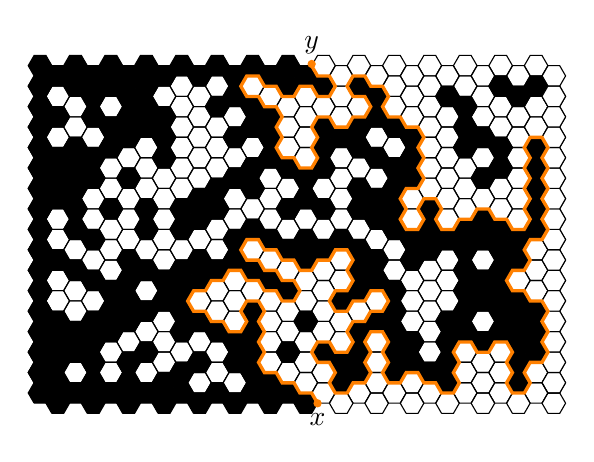
\begin{tikzpicture}
    \begin{scope}[scale=0.15]
      % seed 173
      \foreach \i in {-7,...,7}  {
        \foreach \j in {-7,...,7} {
          \rand
          \draw [fill, fill opacity=\arabic{rand}] (\i*3, \j*1.732) -- ++(0:1) -- ++(60:1) -- ++(120:1) -- ++(180:1) -- ++(240:1) -- ++(300:1);
          \rand
          \draw [fill, fill opacity=\arabic{rand}] (\i*3 + 1.5, \j*1.732 - 0.866) -- ++(0:1) -- ++(60:1) -- ++(120:1) -- ++(180:1) -- ++(240:1) -- ++(300:1);
        }
      }
        \foreach \j in {-7,...,7} {
          \draw [fill] (-7*3, \j*1.732) -- ++(0:1) -- ++(60:1) -- ++(120:1) -- ++(180:1) -- ++(240:1) -- ++(300:1);
          \draw [fill=white] (7*3 + 1.5, \j*1.732 - 0.866) -- ++(0:1) -- ++(60:1) -- ++(120:1) -- ++(180:1) -- ++(240:1) -- ++(300:1);
        }

      \foreach \i in {-7,...,0}  {
        \draw [fill] (\i*3, -8*1.732) -- ++(0:1) -- ++(60:1) -- ++(120:1) -- ++(180:1) -- ++(240:1) -- ++(300:1);
        \draw [fill] (\i*3 + 1.5, -8*1.732 - 0.866) -- ++(0:1) -- ++(60:1) -- ++(120:1) -- ++(180:1) -- ++(240:1) -- ++(300:1);
        \draw [fill] (\i*3, 8*1.732) -- ++(0:1) -- ++(60:1) -- ++(120:1) -- ++(180:1) -- ++(240:1) -- ++(300:1);
        \draw [fill] (\i*3 + 1.5, 8*1.732 - 0.866) -- ++(0:1) -- ++(60:1) -- ++(120:1) -- ++(180:1) -- ++(240:1) -- ++(300:1);
      }
      \foreach \i in {1,...,7}  {
        \draw (\i*3, -8*1.732) -- ++(0:1) -- ++(60:1) -- ++(120:1) -- ++(180:1) -- ++(240:1) -- ++(300:1);
        \draw (\i*3 + 1.5, -8*1.732 - 0.866) -- ++(0:1) -- ++(60:1) -- ++(120:1) -- ++(180:1) -- ++(240:1) -- ++(300:1);
        \draw (\i*3, 8*1.732) -- ++(0:1) -- ++(60:1) -- ++(120:1) -- ++(180:1) -- ++(240:1) -- ++(300:1);
        \draw (\i*3 + 1.5, 8*1.732 - 0.866) -- ++(0:1) -- ++(60:1) -- ++(120:1) -- ++(180:1) -- ++(240:1) -- ++(300:1);
      }

      \node [circ, morange] at (3, -13.866) {};
      \node [below] at (3, -13.866) {$x$};
      \node [circ, morange] at (2.5, 14.866) {};
      \node [above] at (2.5, 14.866) {$y$};

      \draw [morange, very thick] (3, -13.866) -- ++(120:1) -- ++(180:1) -- ++(120:1) -- ++(180:1) -- ++(120:1) -- ++(180:1) -- ++(120:1) -- ++(60:1) -- ++(120:1) -- ++(60:1) -- ++(120:1) -- ++(60:1) -- ++(120:1) -- ++(180:1) -- ++(240:1) -- ++(300:1) -- ++(240:1) -- ++(180:1) -- ++(120:1) -- ++(180:1) -- ++(120:1) -- ++(180:1) -- ++(120:1) -- ++(60:1) -- ++(0:1) -- ++(60:1) -- ++(0:1) -- ++(60:1) -- ++(0:1) -- ++(300:1) -- ++(0:1) -- ++(300:1) -- ++(0:1) -- ++(300:1) -- ++(0:1) -- ++(60:1) -- ++(120:1) -- ++(180:1) -- ++(120:1) -- ++(180:1) -- ++(120:1) -- ++(180:1) -- ++(120:1) -- ++(60:1) -- ++(0:1) -- ++(300:1) -- ++(0:1) -- ++(300:1) -- ++(0:1) -- ++(300:1) -- ++(0:1) -- ++(60:1) -- ++(0:1) -- ++(60:1) -- ++(0:1) -- ++(300:1) -- ++(240:1) -- ++(300:1) -- ++(240:1) -- ++(180:1) -- ++(240:1) -- ++(300:1) -- ++(0:1) -- ++(60:1) -- ++(0:1) -- ++(60:1) -- ++(0:1) -- ++(300:1) -- ++(240:1) -- ++(180:1) -- ++(240:1) -- ++(180:1) -- ++(240:1) -- ++(300:1) -- ++(240:1) -- ++(180:1) -- ++(120:1) -- ++(180:1) -- ++(240:1) -- ++(300:1) -- ++(0:1) -- ++(300:1) -- ++(240:1) -- ++(300:1) -- ++(0:1) -- ++(60:1) -- ++(0:1) -- ++(60:1) -- ++(120:1) -- ++(60:1) -- ++(120:1) -- ++(60:1) -- ++(0:1) -- ++(300:1) -- ++(240:1) -- ++(300:1) -- ++(240:1) -- ++(300:1) -- ++(0:1) -- ++(60:1) -- ++(0:1) -- ++(300:1) -- ++(0:1) -- ++(300:1) -- ++(0:1) -- ++(60:1) -- ++(120:1) -- ++(60:1) -- ++(120:1) -- ++(60:1) -- ++(0:1) -- ++(300:1) -- ++(0:1) -- ++(60:1) -- ++(0:1) -- ++(300:1) -- ++(240:1) -- ++(300:1) -- ++(240:1) -- ++(300:1) -- ++(0:1) -- ++(60:1) -- ++(120:1) -- ++(60:1) -- ++(0:1) -- ++(60:1) -- ++(120:1) -- ++(60:1) -- ++(120:1) -- ++(60:1) -- ++(120:1) -- ++(180:1) -- ++(120:1) -- ++(180:1) -- ++(120:1) -- ++(60:1) -- ++(0:1) -- ++(60:1) -- ++(120:1) -- ++(60:1) -- ++(0:1) -- ++(60:1) -- ++(120:1) -- ++(60:1) -- ++(120:1) -- ++(60:1) -- ++(120:1) -- ++(60:1) -- ++(120:1) -- ++(60:1) -- ++(120:1) -- ++(180:1) -- ++(240:1) -- ++(300:1) -- ++(240:1) -- ++(300:1) -- ++(240:1) -- ++(300:1) -- ++(240:1) -- ++(300:1) -- ++(240:1) -- ++(180:1) -- ++(120:1) -- ++(180:1) -- ++(120:1) -- ++(180:1) -- ++(240:1) -- ++(180:1) -- ++(240:1) -- ++(180:1) -- ++(120:1) -- ++(60:1) -- ++(120:1) -- ++(180:1) -- ++(240:1) -- ++(300:1) -- ++(240:1) -- ++(180:1) -- ++(120:1) -- ++(60:1) -- ++(120:1) -- ++(60:1) -- ++(0:1) -- ++(60:1) -- ++(120:1) -- ++(60:1) -- ++(120:1) -- ++(60:1) -- ++(120:1) -- ++(180:1) -- ++(120:1) -- ++(180:1) -- ++(120:1) -- ++(60:1) -- ++(120:1) -- ++(180:1) -- ++(120:1) -- ++(180:1) -- ++(240:1) -- ++(300:1) -- ++(0:1) -- ++(300:1) -- ++(240:1) -- ++(180:1) -- ++(240:1) -- ++(180:1) -- ++(120:1) -- ++(180:1) -- ++(240:1) -- ++(300:1) -- ++(240:1) -- ++(300:1) -- ++(240:1) -- ++(180:1) -- ++(120:1) -- ++(180:1) -- ++(120:1) -- ++(60:1) -- ++(120:1) -- ++(60:1) -- ++(120:1) -- ++(180:1) -- ++(120:1) -- ++(180:1) -- ++(120:1) -- ++(60:1) -- ++(0:1) -- ++(300:1) -- ++(0:1) -- ++(300:1) -- ++(0:1) -- ++(60:1) -- ++(0:1) -- ++(300:1) -- ++(0:1) -- ++(60:1) -- ++(120:1) -- ++(180:1) -- ++(120:1);
    \end{scope}
  \end{tikzpicture}
\end{center}
Then there exists a unique interface $\gamma_\varepsilon$ that connects $x$ to $y$ with the property that the black hexagons on its left and white on its right. It was conjectured (and now proved by Smirnov) that the limit of the law of $\gamma_\varepsilon$ exists in distribution and is conformally invariant.

This means that if $\tilde{D}$ is another simply connected domain, and $\tilde{x}, \tilde{y} \in \partial \tilde{D}$ are distinct, then $\varphi: D \to \tilde{D}$ is a conformal transformation with $\varphi(x) = \tilde{x}$, $\varphi(y) = \tilde{y}$, then $\varphi(\gamma)$ is equal in distribution of the scaling limit of percolation in $\tilde{D}$ from $\tilde{x}$ to $\tilde{y}$.

Also, percolation also satisfies a natural Markov property: if we condition on $\gamma_\varepsilon$ up to a given time $t$, then the rest of $\gamma_\varepsilon$ is a percolation exploration in the remaining domain. The reason for this is very simple --- the path only determines the colours of the hexagons right next to it, and the others are still randomly distributed independently.

If we assume these two properties, then the limiting path $\gamma$ satisfies the conformal Markov property, and so must be an $\SLE_\kappa$. So the question is, what is $\kappa$?

This is a very common things. We have many discrete model. For some reason, they are supposed to be conformally invariant in the scaling limit and have a Markov property. So we know it is an $\SLE_\kappa$. Then looking at the discrete model, we can deduce some properties about $\gamma$, and this tells us something about which $\kappa$ value it should take.

In the case of percolation, we have the ``locality'' property, and we will see that $\SLE_6$ is the only SLE that satisfies this locality property.

Fix a simply-connected domain $D$ in $\H$ (for simplicity), and assume that $0 \in \partial D$. Suppose we do a percolation exploration in $D$ with black boundary conditions on the clockwise arc of $\partial D$ from $0$ to $y$ and white boundary conditions on the counterclockwise arc. If we think about this a bit, this would be equal in distribution as what we would have got if we performed a percolation exploration on $\H$ with black boundary conditions on $\R_{<0}$ and white boundary conditions on $\R_{>0}$, if we generate the path up until $\partial D \setminus \partial \H$. In other words, $\gamma$ doesn't feel the boundary conditions until it hits the boundary. This is known as \term{locality}.

It should then be true that the corresponding $\SLE_\kappa$ should have an analogous property. To be precise, we want to find a value of $\kappa$ so that the following is true: If $\gamma$ is an $\SLE_\kappa$ in $\H$ from $0$ to $\infty$, run up until it first hits $\partial D \setminus \partial \H$, then $\psi(\gamma)$ is a (stopped) $\SLE_\kappa$ in $\H$ from $0$ to $\infty$ where $\psi: D \to \H$ is a conformal transformation with $\psi(0) = 0$, $\psi(y) = \infty$. This is the \term{locality property}. We will show that locality holds precisely for $\kappa = 6$.

Suppose that $(A_t)$ is a non-decreasing family of compact hulls, parametrized by capacity, locally growing with $A_0 = \emptyset$. In other words, $(A_t) \in \mathcal{A}$. We let
\[
  \tilde{A}_t = \psi(A_t).
\]
The $\tilde{A}_t$ is a family of compact $\H$-hulls that are non-decreasing, locally growing, and $A_0 = \emptyset$. However, in general, this is not going to be parametrized by capacity. Let
\[
  \tilde{a}(t) = \hcap(\tilde{A}_t).
\]
Let $\tilde{g}_T = g_{\tilde{A}_t}$ be the unique conformal transformation $\H \setminus \tilde{A}_t \to \H$ with $\tilde{g}_t(z) - z \to 0$. Then
\[
  \partial_t \tilde{g}_t (z) = \frac{\partial_t \tilde{a}_t}{\tilde{g}_t(z) - \tilde{U}_t},\quad \tilde{g}_0(z),
\]
where $U_t$ is the Loewner driving function for $(A_t)$ and
\[
  \tilde{U}_t = \psi_t(U_t),\quad \psi_t = \tilde{g}_t \circ \psi \circ g_t^{-1},\quad g_t = g_{A_t}.
\]
To see this, recall that if $A_t$ is $\gamma([0, t])$ for a curve $\gamma$, then $U_t = g_t(\gamma(t))$. Then we have
\[
  \tilde{a}(t) = \int_0^t \gamma(\psi_t'(U_s))^2\;\d s.
\]
This is shown in the second example sheet (recall that $\hcap(rA) = r^2 \hcap(A)$). 

We now want to understand what happens when we put $U_t = \sqrt{\kappa} B_t$.
\begin{prop}
  The maps $(\psi_t)$ satisfy
  \[
    \partial_t \psi_t(z) = 2 \left(\frac{(\psi_t'(U_t))^2}{\psi_t(z) - \psi_t(U_t)} - \psi_t' (U_t) \frac{1}{z - U_t}\right).
  \]
  In particular, at $z = U_t$, we have
  \[
    \partial_t \psi_t(U_t) = \lim_{z \to U_t} \partial_t \psi_t (z) = -3 \psi_t''(U_t).
  \]
\end{prop}



\printindex
\end{document}
